% School Dynamics — Milestone 4 Report
% Compile from repository root: pdflatex MILESTONE4_REPORT.tex (run twice for TOC)
% Requires: docs/wireframes/figma-wireframes-part1.png … part3.png
%           (regenerate via scripts/capture-figma-wireframe-screenshots.sh)

\documentclass[11pt,a4paper]{article}

\usepackage[utf8]{inputenc}
\usepackage[T1]{fontenc}
\usepackage{lmodern}
\usepackage[margin=1in]{geometry}
\usepackage{graphicx}
\usepackage{booktabs}
\usepackage{hyperref}
\usepackage{enumitem}
\usepackage{xcolor}

\hypersetup{
  colorlinks=true,
  linkcolor=blue!60!black,
  urlcolor=blue!60!black,
  citecolor=blue!60!black,
  pdftitle={School Dynamics --- Milestone 4 Report},
  pdfauthor={Project Team}
}

\title{\textbf{School Dynamics}\\[0.35em]
\large Milestone 4: Web Application, Portals, and Delivery Readiness}
\author{School Dynamics Project}
\date{\today}

% ------------------------------------------------------------------
% Published marketing landing page (GitHub Pages)
% ------------------------------------------------------------------
\newcommand{\PublishedLandingURL}{https://genoj83.github.io/School-Dynamics/}
\newcommand{\WireframesURL}{https://visor-unity-00479441.figma.site/}

\begin{document}

\maketitle

\begin{abstract}
\noindent
This report documents Milestone~4 for \textbf{School Dynamics}, a school management solution oriented toward Ugandan institutions. The milestone delivers a responsive web application with distinct \emph{staff} and \emph{parent} portals, a public landing experience with a clear unique value proposition (UVP), client-side data workflows suitable for demonstration and iteration, supporting documentation for marketing and design handoff, and alignment with common submission criteria including SEO basics and feature traceability.

\vspace{0.5em}
\noindent\textbf{Live landing page:} \href{\PublishedLandingURL}{\texttt{\PublishedLandingURL}}

\vspace{0.35em}
\noindent\textbf{High-fidelity wireframes (Figma site):} \href{\WireframesURL}{\texttt{\WireframesURL}}
\end{abstract}

\tableofcontents
\newpage

%----------------------------------------------------------------------
\section{Introduction and milestone scope}

\subsection{Project context}
School Dynamics is conceived as an integrated platform for student records, fee management, attendance, examinations, and communication, with explicit support for \textbf{staff operations} and a \textbf{parent-facing} read model. Milestone~4 focuses on \textbf{front-end realization}, \textbf{dual-portal information architecture}, and \textbf{packaging} of deliverables for stakeholders (including coursework or sponsor review).

\subsection{Objectives addressed in Milestone~4}
The following objectives guide this milestone:
\begin{enumerate}[leftmargin=*]
  \item Implement a \textbf{live-buildable} web application with navigable staff and parent journeys.
  \item Present a \textbf{clear UVP} at the entry experience (landing and sign-in copy).
  \item Ensure \textbf{mobile-responsive} layouts for primary flows.
  \item Maintain \textbf{basic SEO} metadata at the application shell level.
  \item Produce \textbf{documentation} suitable for a marketing video script and for \textbf{Figma} wireframe generation.
  \item Enumerate \textbf{five to seven core solution features} with mapping to implemented screens.
\end{enumerate}

\subsection{Repository structure (high level)}
\begin{itemize}[leftmargin=*]
  \item \texttt{/index.html}, \texttt{style.css}, \texttt{script.js}, \texttt{assets/} --- standalone marketing landing (legacy path in repository root).
  \item \texttt{/webapp/} --- React + TypeScript + Vite application: landing route, staff portal, parent portal, shared client-side school data layer.
\end{itemize}

%----------------------------------------------------------------------
\section{Unique value proposition (UVP)}

The UVP is expressed consistently as: \textbf{one school platform with two purposeful entry points} --- staff run day-to-day operations; parents access fees, attendance, and grades without administrative clutter. The in-app landing page (\texttt{/}) foregrounds this split and routes users to \texttt{/login} (staff) or \texttt{/parents/login} (parents).

%----------------------------------------------------------------------
\section{Technical summary}

\subsection{Stack}
\begin{itemize}[leftmargin=*]
  \item \textbf{Framework:} React~19 with TypeScript.
  \item \textbf{Build tool:} Vite.
  \item \textbf{Routing:} React Router.
  \item \textbf{State and persistence:} React context; school records persisted in \texttt{localStorage} under a versioned key for demonstration (replaceable with API integration).
  \item \textbf{Styling:} Global CSS with design tokens (accent \texttt{\#C70039}, parent portal teal accent, responsive breakpoints).
\end{itemize}

\subsection{Authentication model (current)}
\begin{itemize}[leftmargin=*]
  \item \textbf{Staff:} Email-based session stored locally; suitable for prototype sign-in flows.
  \item \textbf{Parents:} Lookup by admission number or normalized phone digits matched against student records; session stored separately from staff.
\end{itemize}

%----------------------------------------------------------------------
\section{Core features (seven) and implementation mapping}

Table~\ref{tab:features} lists seven core features and their primary UI location in the \texttt{webapp} source.

\begin{table}[h]
  \centering
  \caption{Core features and primary routes/components}
  \label{tab:features}
  \begin{tabular}{@{}p{0.06\textwidth}p{0.34\textwidth}p{0.48\textwidth}@{}}
    \toprule
    \textbf{\#} & \textbf{Feature} & \textbf{Implementation notes} \\
    \midrule
    1 & Dual-portal landing & \texttt{LandingPage.tsx}, routes \texttt{/} \\
    2 & Staff dashboard & \texttt{/app/dashboard}, \texttt{DashboardHome.tsx} \\
    3 & Student registry & \texttt{/app/students}, \texttt{Students.tsx}, detail \texttt{StudentDetail.tsx} \\
    4 & Fee invoices (UGX) & \texttt{/app/fees}, \texttt{Fees.tsx} \\
    5 & Attendance by date & \texttt{/app/attendance}, \texttt{Attendance.tsx} \\
    6 & Exams / gradebook & \texttt{/app/exams}, \texttt{Exams.tsx} \\
    7 & Parent portal (fees, attendance, grades) & \texttt{/parents/*}, \texttt{pages/parent/} \\
    \bottomrule
  \end{tabular}
\end{table}

\noindent
\textbf{Additional capability:} a \textbf{messages} log (\texttt{/app/messages}) supports communication tracking; parent views remain read-focused for fees, attendance, and published grades.

%----------------------------------------------------------------------
\section{Responsive design}

Layouts use flexible grids, collapsible navigation patterns on narrow viewports, and a mobile-friendly top bar on staff and parent shells. The landing page uses responsive portal cards (side-by-side on wide screens, stacked on small screens). Manual verification is recommended on representative devices (e.g.\ 390\,px and 1440\,px widths) before final submission recordings.

%----------------------------------------------------------------------
\section{SEO and discoverability}

\subsection{Application shell (\texttt{webapp/index.html})}
The Vite shell includes a document \textbf{title}, \textbf{meta description}, and viewport configuration appropriate for a progressive web client.

\subsection{Marketing page (repository root)}
The standalone \texttt{index.html} includes extended metadata: keywords, Open Graph and Twitter card tags, and canonical URL placeholder aligned with the School Dynamics brand domain used in marketing materials.

\subsection{Headings}
Primary views use hierarchical headings (\texttt{h1}/\texttt{h2}) for structure within the React application, supporting both accessibility and content outline clarity.

%----------------------------------------------------------------------
\section{Documentation and design handoff}

\subsection{Marketing video}
\texttt{MARKETING\_VIDEO.md} contains a scene-by-scene \textbf{voiceover script} with visual cues and approximate timing, suitable for recording a milestone or promotional video.

\subsection{Figma wireframes}
High-fidelity wireframes for primary user flows are published at:

\begin{center}
\href{\WireframesURL}{\texttt{\WireframesURL}}
\end{center}

\noindent
The repository file \texttt{FIGMA\_AI\_WIREFRAME\_PROMPT.md} retains the structured prompt used to guide wireframe generation (desktop and mobile frames, staff and parent flows).

\noindent
\textbf{Embedded screenshots:} Full-width captures from the live Figma site appear in Appendix~\ref{app:wireframes} (parts 1--3), so the report remains self-contained when printed or submitted as PDF.

%----------------------------------------------------------------------
\section{Deployment note (published URL)}

The \textbf{public landing page} for this milestone is available at:

\begin{center}
\href{\PublishedLandingURL}{\texttt{\PublishedLandingURL}}
\end{center}

\noindent
The application was produced by building the \texttt{webapp} package (\texttt{npm run build} $\rightarrow$ \texttt{dist/}) and deploying static assets to a hosting provider (e.g.\ Netlify, Vercel, Cloudflare Pages, GitHub Pages). The repository remains \textbf{deployment-ready} for updates; change the URL macro in the preamble of this document if the hostname changes.

%----------------------------------------------------------------------
\section{Limitations and next milestone directions}

\begin{itemize}[leftmargin=*]
  \item \textbf{Backend:} No production API or database in this milestone; data is browser-local for demonstration.
  \item \textbf{Security:} Staff and parent authentication are not enterprise-grade; production requires identity provider integration, authorization, and audit policies.
  \item \textbf{Design artifacts:} Wireframes are available at the Figma site above; source files may still live in Figma for editing per course instructions.
  \item \textbf{Analytics:} No third-party analytics SDK is embedded; adoption metrics would be a later integration.
\end{itemize}

%----------------------------------------------------------------------
\section{Conclusion}

Milestone~4 delivers a \textbf{coherent dual-portal web application}, \textbf{documented core features}, \textbf{responsive UI patterns}, \textbf{baseline SEO} in the HTML shell, and \textbf{supporting artifacts} for video and wireframe production. The solution is positioned for Milestone~5 (or equivalent) work: backend services, real authentication, hosting at a stable public URL, and formal usability testing.

%----------------------------------------------------------------------
\appendix
\section{Wireframe screenshots}
\label{app:wireframes}

\noindent
These figures are \textbf{automated full-page captures} of the published high-fidelity wireframes at \href{\WireframesURL}{\texttt{\WireframesURL}}, split into three vertical bands for legible printing. Layout order follows the primary user flow: portal selection and staff journey (part~1), staff dashboard and related screens (part~2), parent journey (part~3).

\begin{figure}[p]
  \centering
  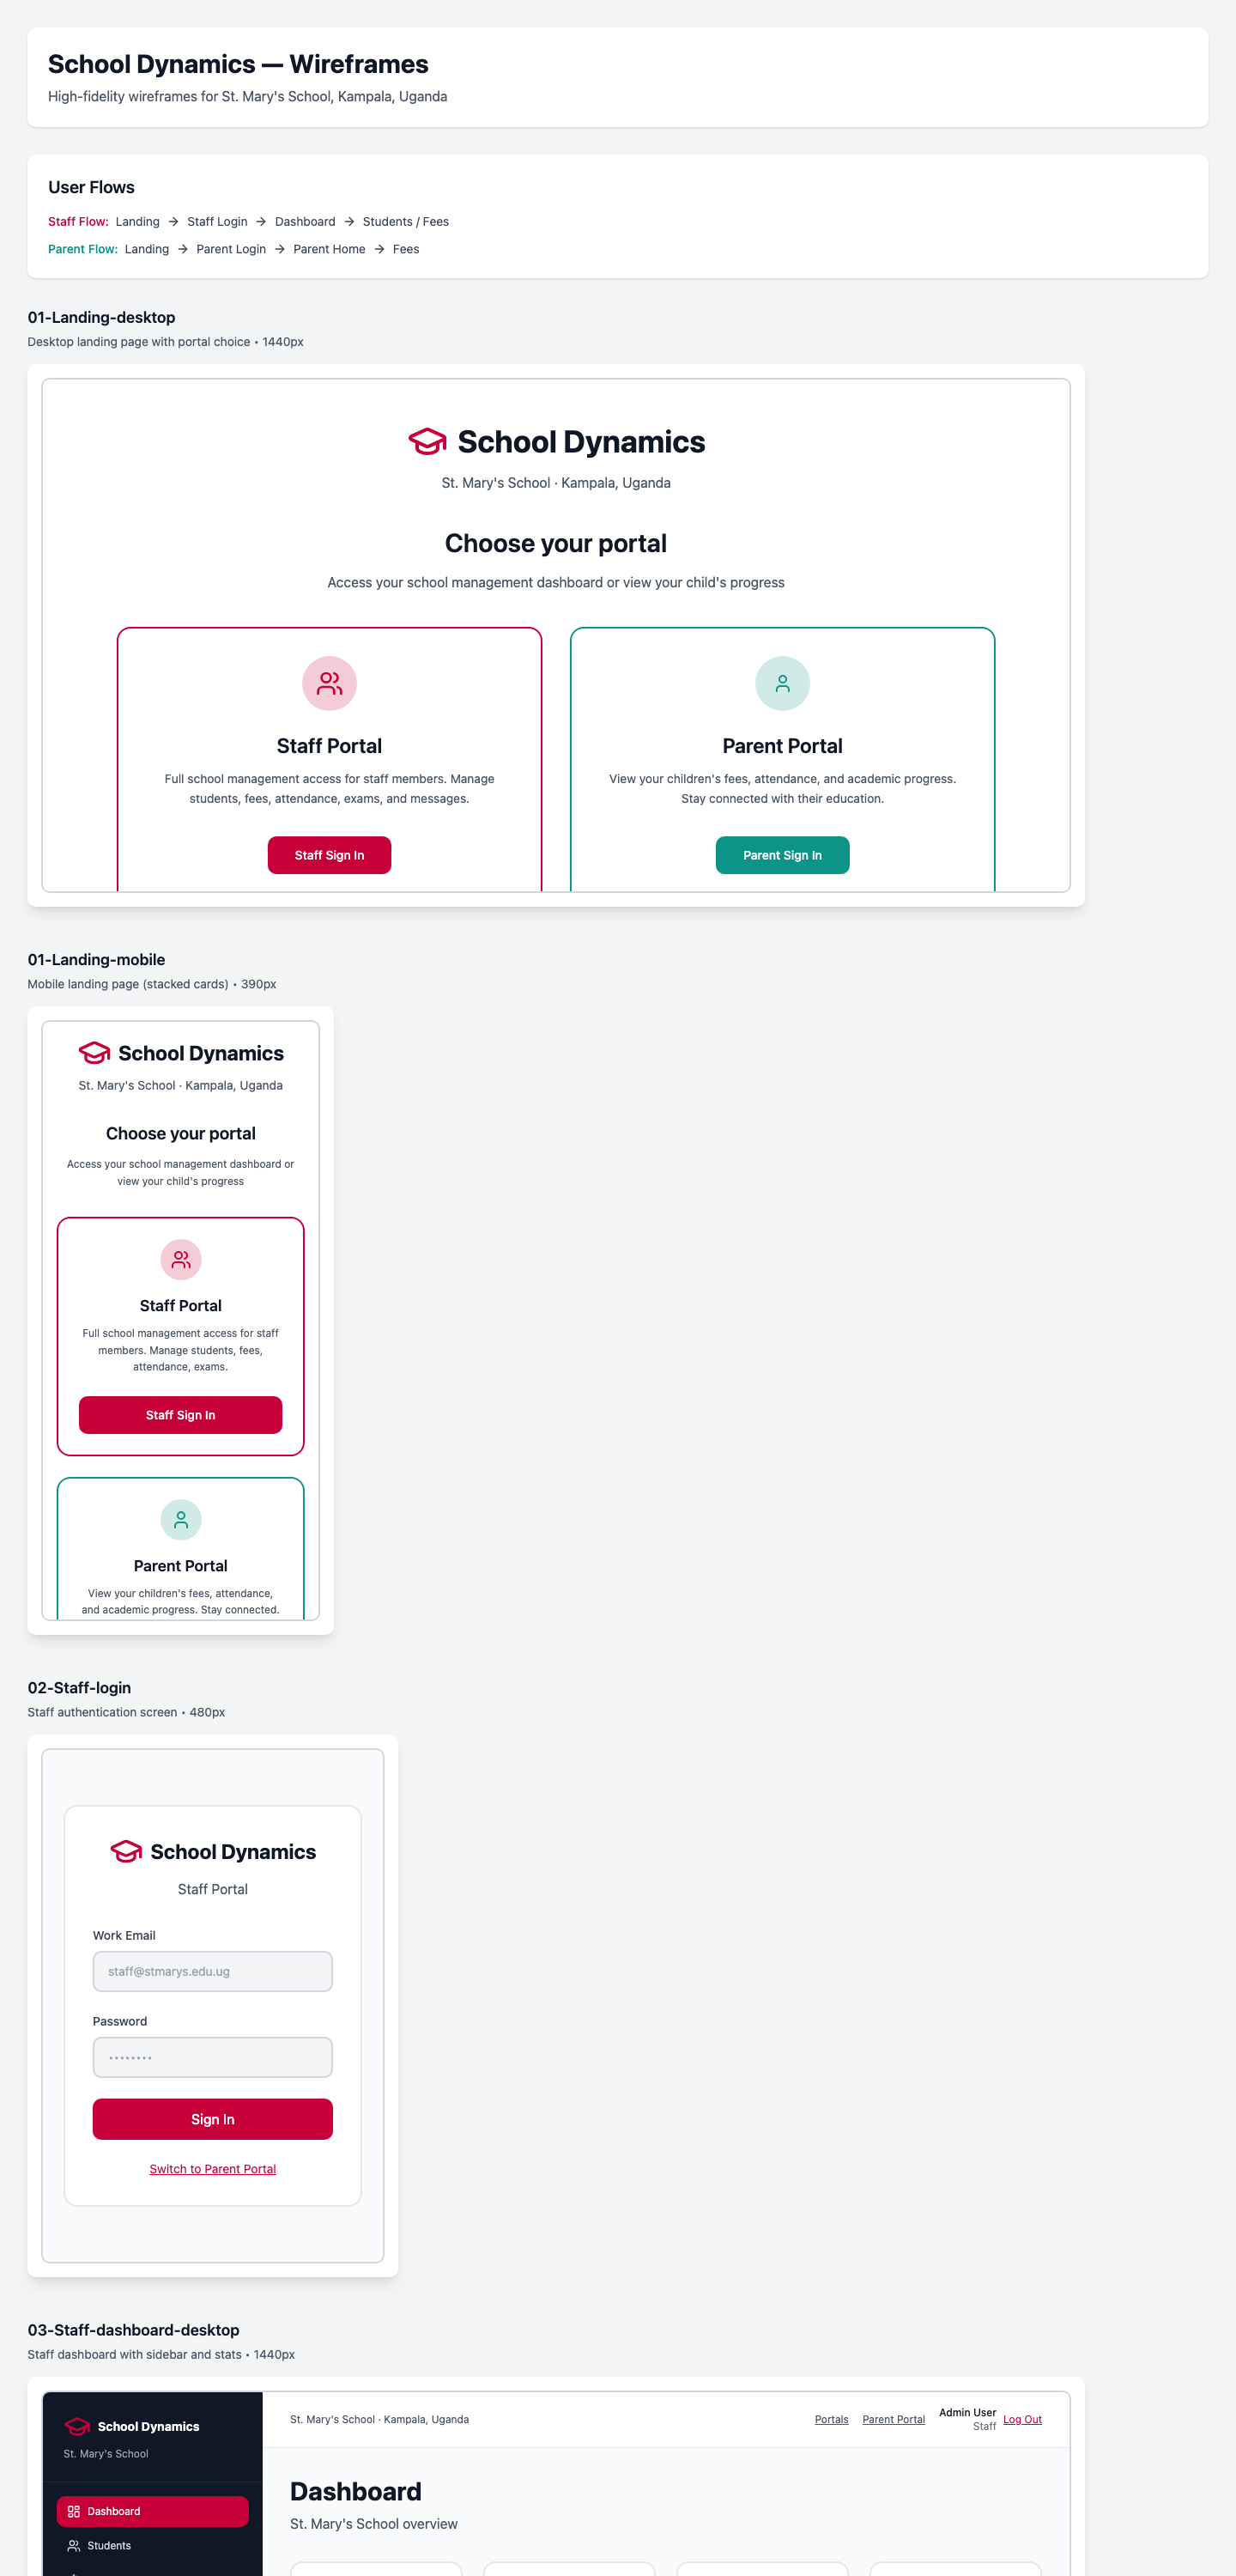
\includegraphics[width=\textwidth]{docs/wireframes/figma-wireframes-part1.png}
  \caption{Wireframes (part 1 of 3): portal landing (desktop/mobile) and staff entry.}
  \label{fig:wire-a}
\end{figure}

\begin{figure}[p]
  \centering
  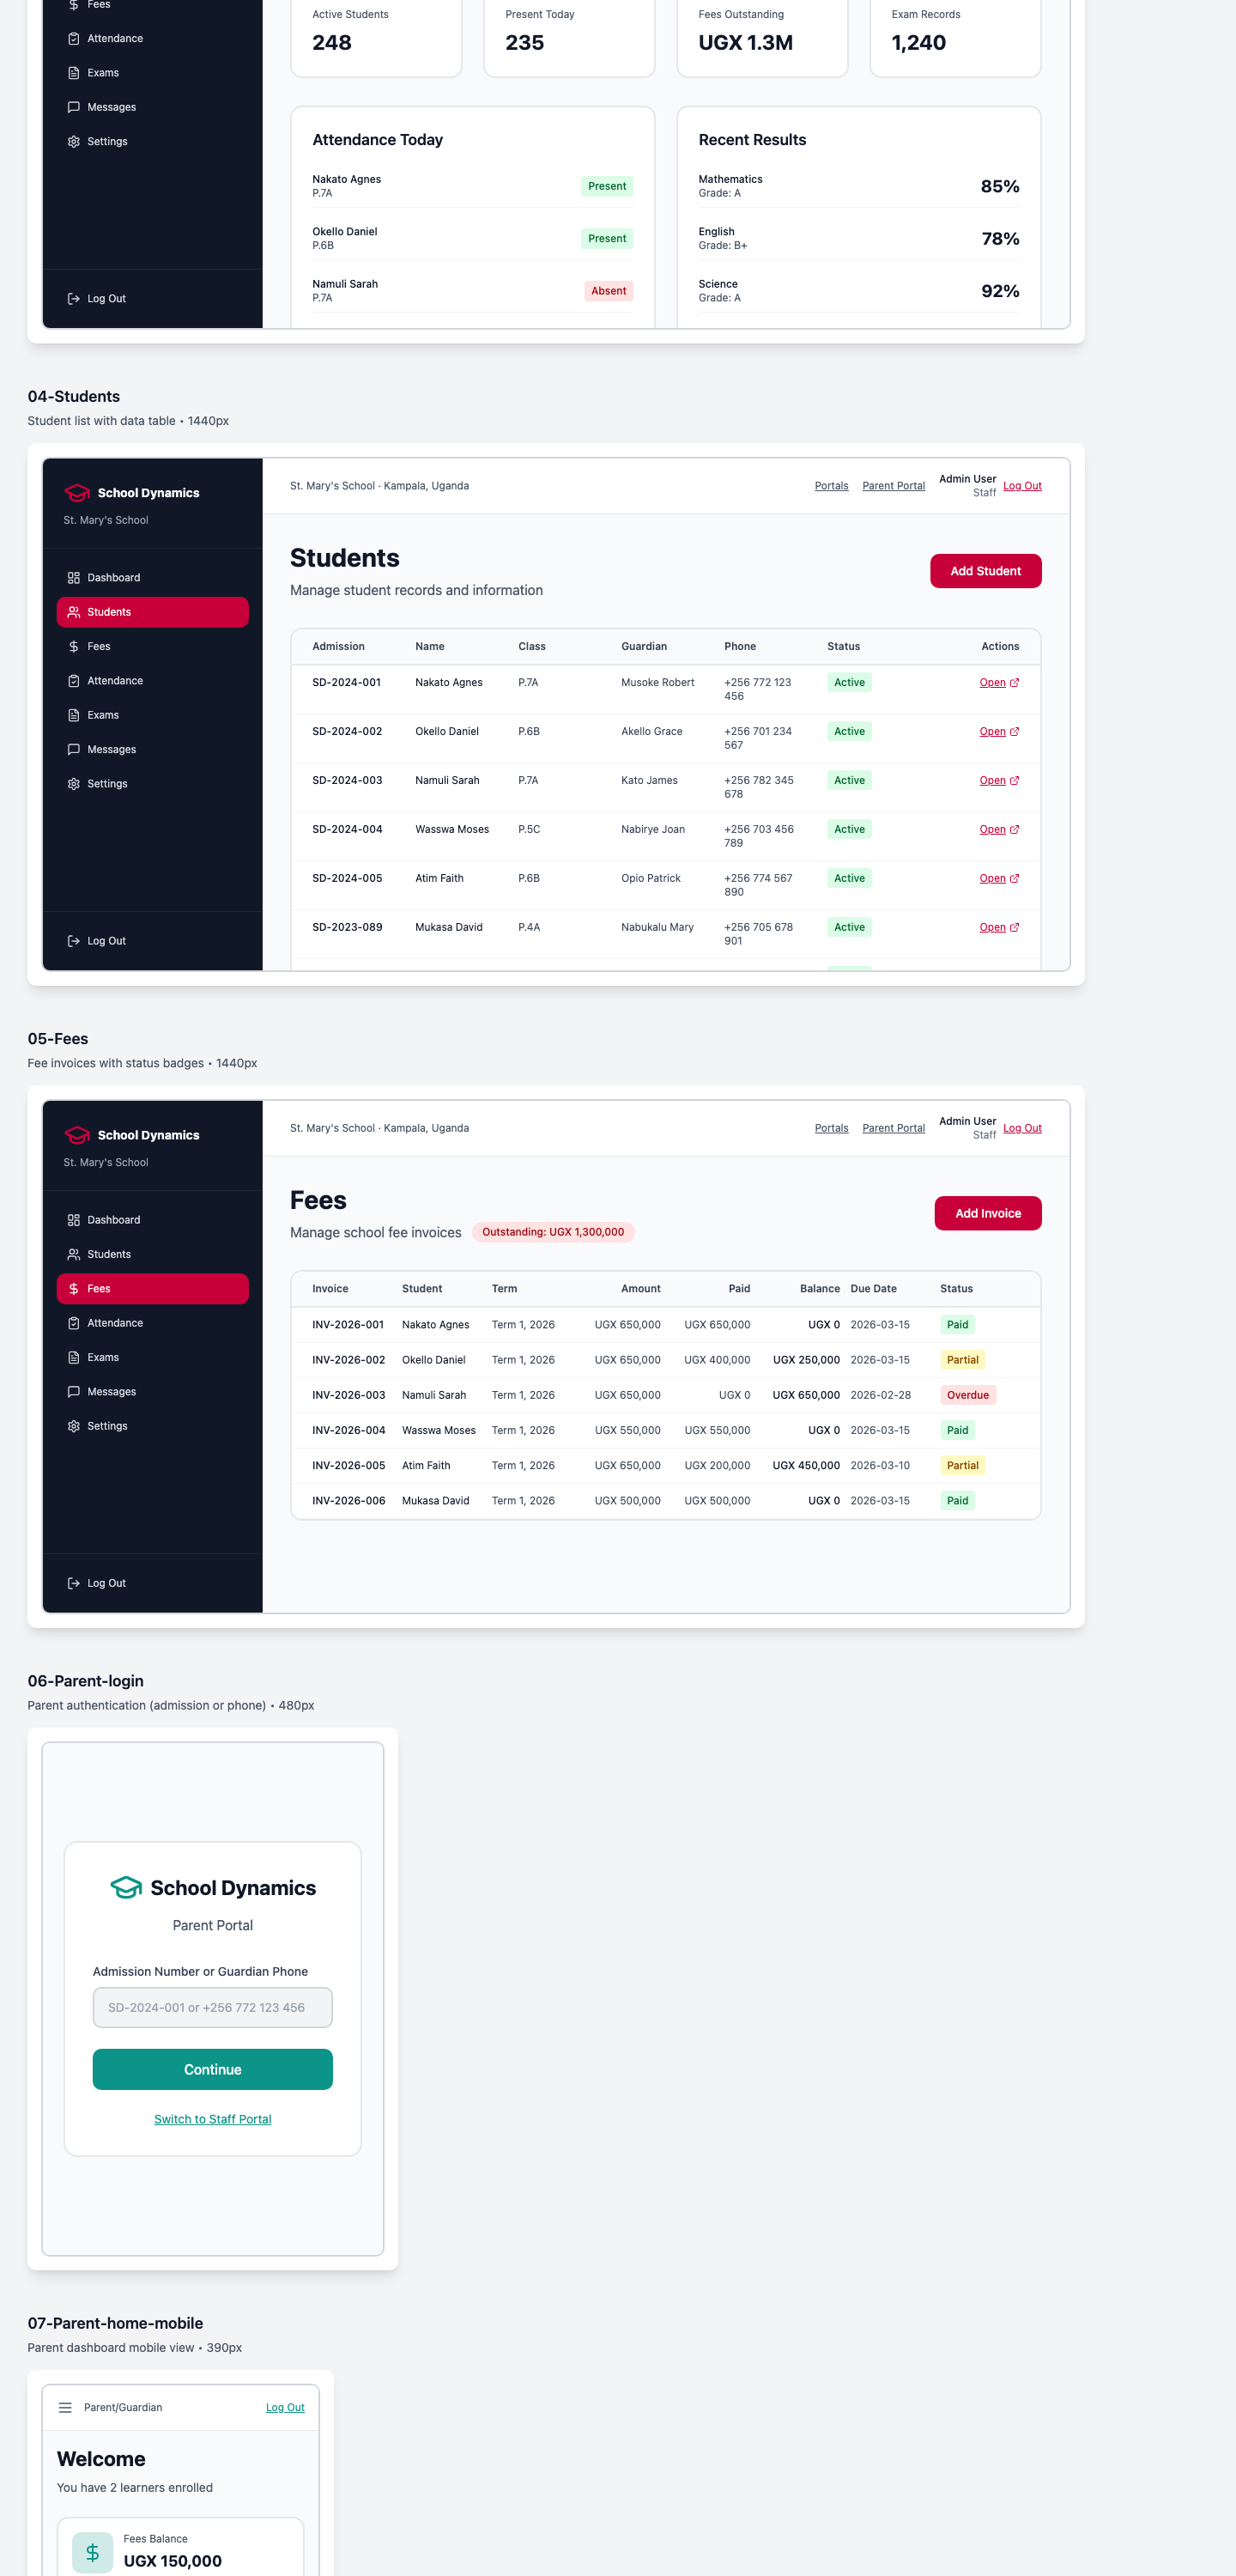
\includegraphics[width=\textwidth]{docs/wireframes/figma-wireframes-part2.png}
  \caption{Wireframes (part 2 of 3): staff dashboard, students, and fees.}
  \label{fig:wire-b}
\end{figure}

\begin{figure}[p]
  \centering
  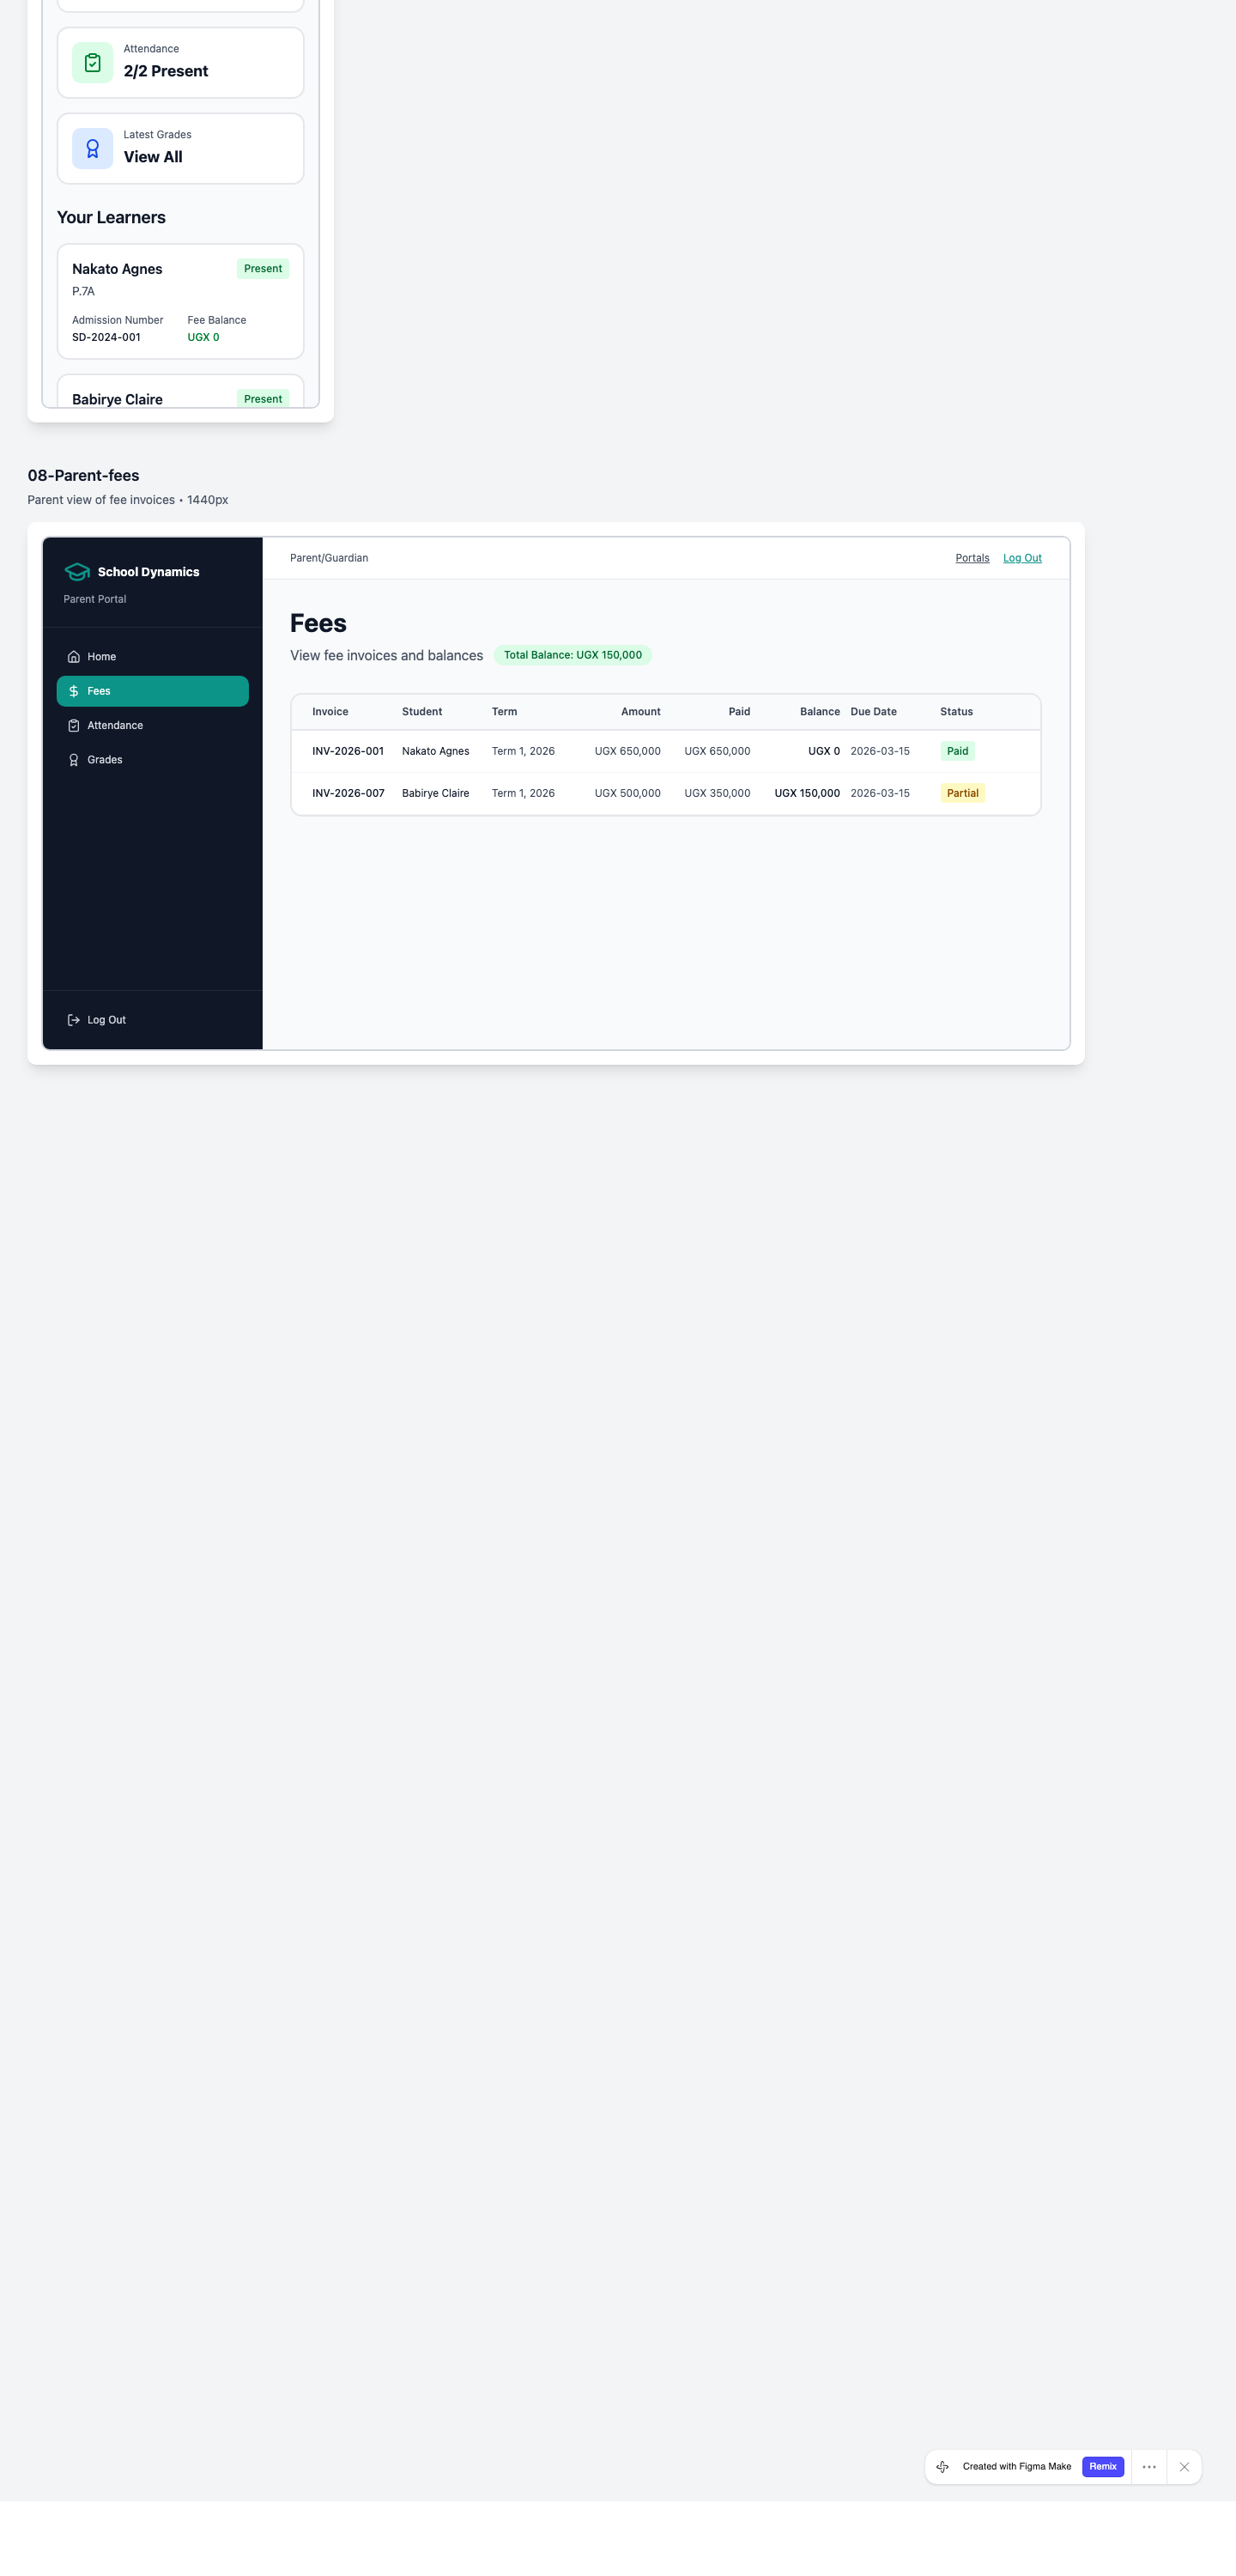
\includegraphics[width=\textwidth]{docs/wireframes/figma-wireframes-part3.png}
  \caption{Wireframes (part 3 of 3): parent sign-in, parent home, and parent fees.}
  \label{fig:wire-c}
\end{figure}

\vspace{1em}
\noindent\textbf{Build reference (web application):}
\begin{verbatim}
cd webapp && npm install && npm run build
\end{verbatim}

\end{document}
